%\documentclass[11pt]{article}
%\usepackage[a4paper, total={6.5in, 9.5in}]{geometry}
%\usepackage[document]{ragged2e}
%\usepackage{lipsum}
%\usepackage{graphicx}
%\usepackage{float}
%\usepackage{multirow}
%\usepackage{array}
%\usepackage{cellspace}
%\usepackage{etoolbox}
%\usepackage{scrpage2}
%\usepackage{longtable}
%\usepackage[table, svgnames]{xcolor}
%\usepackage{titlesec}
%\setcounter{secnumdepth}{4}
%\titleformat{\paragraph}
%{\normalfont\normalsize\bfseries}{\theparagraph}{1em}{}
%\titlespacing*{\paragraph}
%{0pt}{3.25ex plus 1ex minus .2ex}{1.5ex plus .2ex}
%\ifoot[]{}
%\cfoot[]{}
%\ofoot[\pagemark]{\pagemark}
%\pagestyle{scrplain}
%\begin{document}

\setcounter{section}{1}
\section{System Overview}
\bigskip
\subsection{System Layout}
\bigskip
The Akriveia Beacon indoor locating rescue system combines electrical, hardware and software systems to detect and locate multiple occupants within a building during an emergency disaster situation. Each individual component of the system is developed separately in the PoC (Proof of Concept) phase; then partially integrated in the Prototype phase and fully integrated in the Final Product phase.

\bigskip
A high-level system overview displays three Locator Beacons, an ID tag, a Server and a user interface (Figure \ref{fig:system_layout}).
The Locator Beacons transmits wireless signals to the Access Card to acquire a response.
When the beacons receive a response back, the received signal data will be forwarded to the data processing server to calculate the distance and location of the ID tag through trilateration algorithms.
Afterwards, the location results are displayed on a \Gls{GUI} for operators.


\begin{figure}[h!]
    \centering
    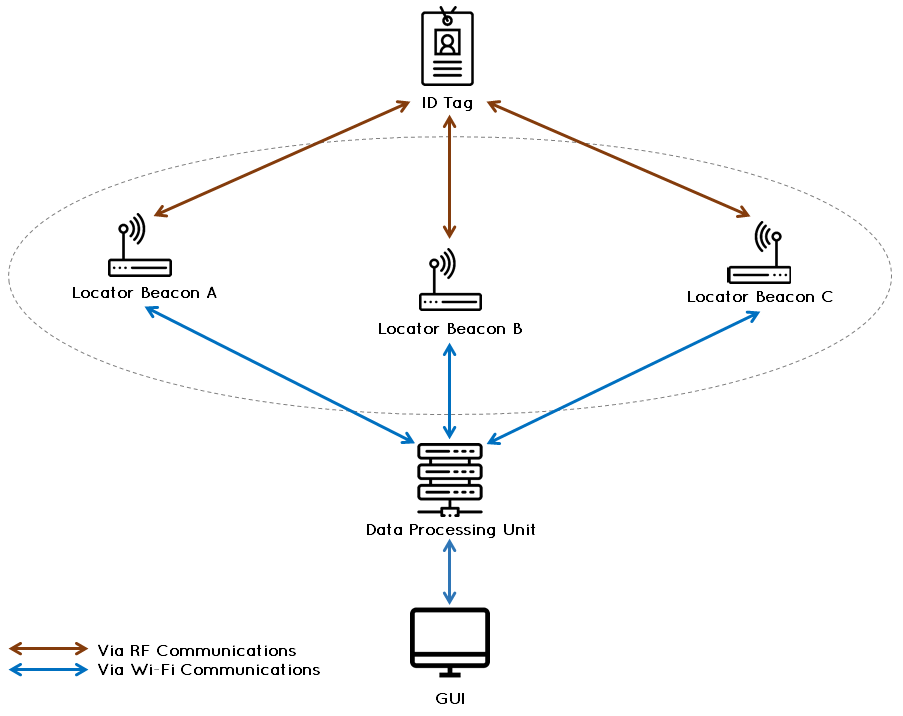
\includegraphics[width=\linewidth]{./images/00_sys_arch.png}
    \caption{System Layout Overview}
    \label{fig:system_layout}
\end{figure}


\break
\subsubsection{Proof Of Concept (PoC)}

\bigskip
The Proof of Concept (\Gls{PoC}) demonstrates the feasibility of the location determination system using Beacons to ID tag distances estimation along with trilateration. Such a system should show the effectiveness of a trilateration algorithm for determining distance and location of the ID tag in 2 dimensional space. For the PoC, all equipment are powered by a external power supply; as the main goal of the PoC is to demonstrate the feasibility of locating access card with location beacon system with trilateration algorithms.

\begin{figure}[h!]
    \centering
    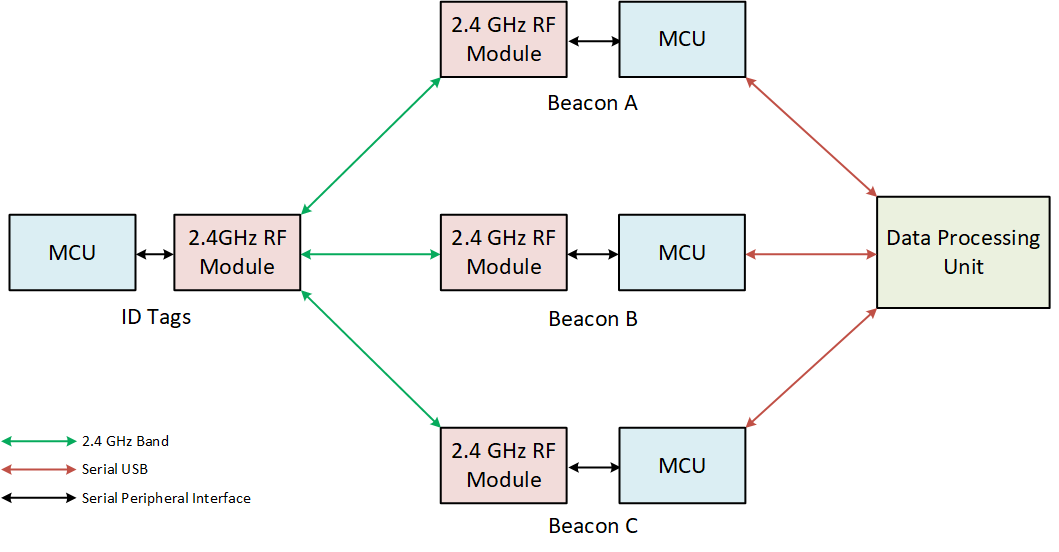
\includegraphics[width=\linewidth]{./images/01_sys_PoC.png}
    \caption{PoC System Block Diagram}
    \label{fig:PoC_sys_blk}
\end{figure}
\bigskip

This system will use four 2.4 GHz \Gls{RF} modules, four micro-controller units (\Gls{MCU}) and a Raspberry Pi as the data processing server. The proof-of-concept demonstrates the following objectives:

\begin{enumerate}
    \item Utilization of 2.4 GHz RF module chips as signal receiver and transmitter
    \item Establish functioning RF data communication between the RF modules with one module as the ID tag and three as the locator beacons
    \item Perform radio fingerprinting process to determine transmitter properties such as RSSI, time of flight (\Gls{ToF}), and other data
    \item Send distance data from the location beacons to the server for data processing
    \item Implement trilateration algorithms using distance estimation to determine ID card location in 2D space
\end{enumerate}

\break
\subsubsection{Prototype}
\bigskip
The Prototype demonstrates the same objectives from the PoC except the transceivers will be using Ultra-wideband (UWB) signals instead of 2.4 GHz band signals. UWB uses the radio frequencies of 3.5 to 6.5 GHz and would significantly reduce the issue of signal interference or multipath propagation. Although 2.4 GHz is more widely used for its versatility, UWB would be more well suited for the Akriveia Beacon system. Selecting UWB chips would result in a higher wave propagation effect, lower signal interference and signal multipath \cite{R4}. In additional, an early prototype RF harvesting circuit would be implemented during the prototype phase to test the feasibility of the concept.

\begin{figure}[h!]
    \centering
    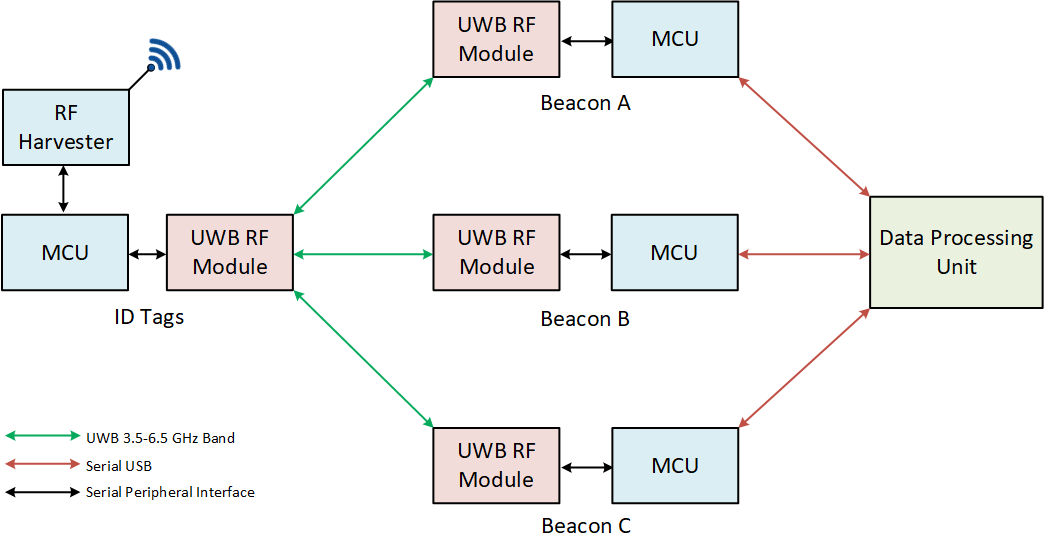
\includegraphics[width=\linewidth]{./images/02_sys_Prototype.png}
    \caption{Prototype System Block Diagram}
    \label{fig:prototype_sys_blk}
\end{figure}
\bigskip

The objectives of the Prototype remains largely the same with the PoC besides using UWB
chips and developing RF harvester circuit. Prototype phase objectives are stated below:

\begin{enumerate}
    \item Utilizing UWB RF module chips in the UWB frequencies of 3.5 to 6.5 GHz as
    signal receivers and transmitters
    \item Establishing functioning RF data communication between the four UWB modules
    with one as the Access Card and three as the Locator Beacons
    \item Using signal fingerprinting to determine transmitter properties such as ToF,
    RSSI and unique identifier
    \item Implement manual off/on activation switch to RF module circuit on ID tags
    \item Apply trilateration algorithms on data processing server to determine
    ID card location
    \item Implementation of software stack on server and initial development of GUI
    \item Prototype and early implementation of  RF harvesting circuit or device charging
\end{enumerate}

\break
\paragraph{RF Harvester Prototype Design}
\bigskip
RF is an abundant source for energy harvesting especially in a radio wave rich environment. When Radio Waves reach an antenna it causes a changing potential difference across the antenna. The potential difference causes charge carriers to move along the length of the antenna in an attempt to equalize the field, and the RF to \Gls{DC} integrated circuit (Figure \ref{fig:rfh}) is able to capture energy from the movement of those charge carriers. The energy is stored temporarily in a capacitor and then used to create a desired potential difference at the load \cite{R5}.
\begin{figure}[h!]
    \centering
    \includegraphics[width=\linewidth]{./images/rf_harvest.png}
    \caption{Prototype System Block Diagram}
    \label{fig:rfh}
\end{figure}

\bigskip
There will be a demonstrable RF harvester circuit similar to Figure \ref{fig:rfh} that would convert ambient radio signal to DC voltage to charge the ID tag battery. The harvester will operate at the standard 2.4 GHz band as ambient RF signal is most comment at this frequency (ie. WiFi, Cellular). The received signal would be put through a rectifier to generate a DC voltage. Through the RF harvester circuit the RF signal power would be transferred to the circuit battery to maintain charge. The yield of the power generated would be small but the effect would be constant in an RF rich environment.

\break
\subsubsection{Final Product}
\bigskip
The final product will demonstrate the final fully functional indoor rescue system that detects the location of the ID tags and displays it accordingly on a GUI. All the components of the systems will be fully integrated as a close-to-production product. Component circuit and \Gls{PCB} footprint will be minimized and proper casing will be made to house all electronics. The data processing server will provide the user with a full GUI to interact with the system along with the fully implemented features such as importable blueprints and multi-floor tacking.

\begin{figure}[h!]
    \centering
    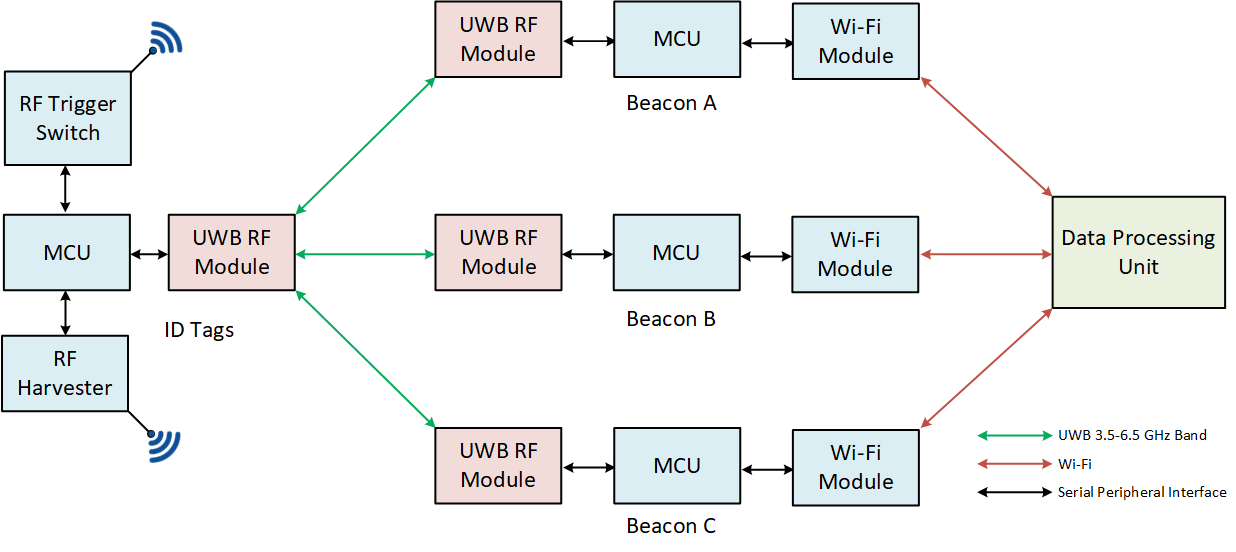
\includegraphics[width=\linewidth]{./images/03_sys_Final.png}
    \caption{Final Product System Block Diagram}
    \label{final_prod_sys_blk}
\end{figure}
\bigskip

The final product should satisfy these objectives below:

\begin{enumerate}
    \item Establishing functioning RF data communication between the four UWB modules with
    one imitating the Access Card and three imitating the Locator Beacons
    \item Using signal fingerprinting to determine transmitter properties such as ToF, RSSI
    and unique identifier
    \item Utilizing UWB RF module chips in the frequencies of 3.5 to 6.5 GHz as signal receivers/transmitters
    \item Develop an ID tag with manual (ON) RF module activation, one RF harvesting circuit
    for charging and one RF harvester as a RF Trigger switch
    \item Send the data to the server to be processed
    \item Have the data processing server apply trilateration algorithms to determine ID card location
    \item Optimize trilateration algorithms to increase accuracy and speed of location calculation
    \item Display locations on a intuitive GUI for the user
\end{enumerate}

\break
\paragraph{RF Harvester Final Design}
\bigskip
Once RF harvester test circuit produces adequate results in the prototype phase, there will be two RF harvester circuits implemented on the ID tags in the final design. The primary RF harvester will act as a RF trigger switch to activating the RF module in case of an emergency, the second RF harvester will be for for charging the ID tags using ambient RF signals.

\bigskip
The first RF harvester circuit will activate the ID tag RF module circuit, this harvester will operate
on a different frequency and power level, making it distinguishable from UWB or other ambient radio frequencies. The second RF harvester circuit designed for charging the ID tags will be operating at the standard 2.4 GHz band  as ambient RF signal is most comment at this frequency (i.e. Wi-Fi, Cellular). The charging RF harvester would have been implemented and tested in the prototype phase. Minor modification and optimization of the circuit would occur in the final phase.

\bigskip
Both RF harvester circuits will be integrated together with the RF module circuit together as an ID tag.

\break
\subsection{Trilateration Overview}
\bigskip
\subsubsection{Proof of Concept (PoC)}
\bigskip
The Akriveia Beacon System will employ a two dimensional trilateration positioning method to locate the mobile sensors within the ID tags in the Proof-of-Concept (PoC) phase as shown in Figure \ref{Tri}. The method will abide the scheme of lateration with absolute distances, which uses distance-related measurements to describe the distance between mobile sensors and several fixed sensors. The metric to be used for distance-related measurements will be Time-of-Flight (ToF), which describes the signal propagation time in a one way communication between a transmitter and a receiver \cite{R6}. In the PoC phase, ToF data will be collected from 2.4 GHz RF medium and converted to distance based on a form of Distance Speed Time formula.

\bigskip
\begin{figure}[h!]
    \centering
    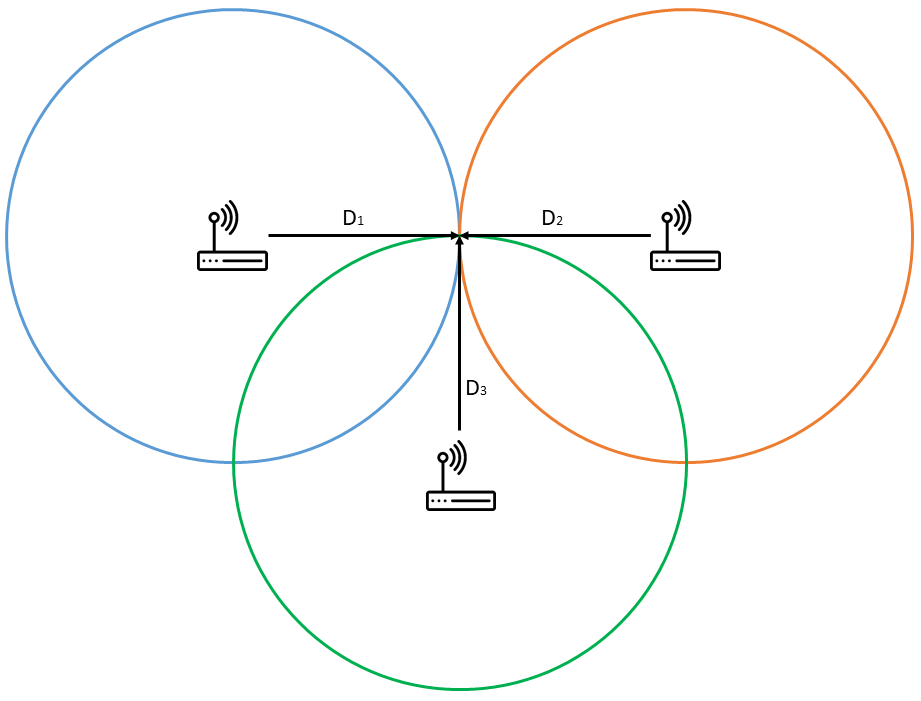
\includegraphics[width=\linewidth]{./images/Tri.png}
    \caption{Trilateration Diagram}
    \label{Tri}
\end{figure}
\bigskip

\begin{equation}
D_n = 10^{(Measured Power - RSSI)/10N}
\end{equation}
Measured Power - Expected RSSI at a distance of one meter (factory calibrated)
N - Environmental factor, range from 2 to 4


\subsubsection{Prototype/Final Product}
In the Engineering Prototype and Final Product phase, the Akriveia Beacon System will not only continue to adhere to the concept of lateration with absolute distances for positioning computation, but also extend its application into three dimensions. In combating the vulnerability of signals being multipathed in a 2.4 GHz RF medium, the transceiver modules of the beacons and ID tags will be replaced with ultra-wideband (UWB) modules, where operational UWB frequencies ranges from 3.5 GHz to 6.5 GHz \cite{R42}.
\break



\subsection{Software System Overview}
\bigskip
Akriveia's software design is specifically chosen for safety, robustness and performance. It's primary compute server is powered by a Raspberry Pi 3 B+ running a Rust web server to leverage type-safety and memory access guarantees while still maintaining C++ like performance because of compiled binaries and lack of garbage collection. Figure \ref{software_diagram} below is a diagram of the software architecture, which serves content through the web server to first responders while processing real time location data of users from beacons in the background. The server will make use of the widely used model-view-controller architecture to reduce development costs and leverage modern software development practices. Sqlite was chosen for its simplicity and minimal system footprint, which is intended to be used to persist data such as user and beacon location information, and building blueprints.

\bigskip
\begin{figure}[h!]
    \centering
    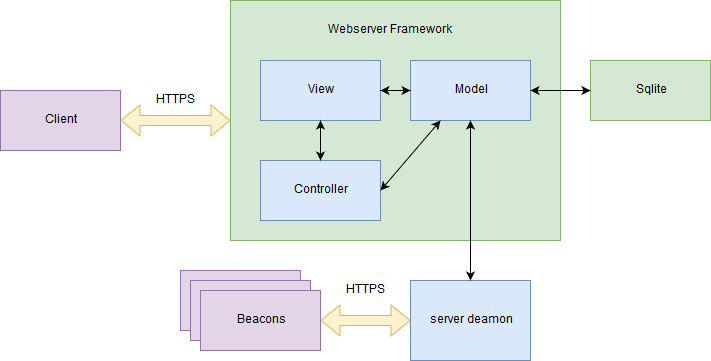
\includegraphics[width=\linewidth]{./images/softwarediagram.png}
    \caption{Akriveia Software Overview}
    \label{software_diagram}
\end{figure}
\bigskip


%\end{document}
